%%%%%%% Preambule %%%%%%%%
% třída dokumentu
\documentclass[12pt,a4paper,hidelinks]{article}

% kvůli písmům a ligaturám (např. --)
% toto je pro XeLaTeX!
\usepackage{fontspec}
\defaultfontfeatures{Mapping=tex-text}
\usepackage{xunicode}
\usepackage{xltxtra}
\setmainfont{Times New Roman}

% nastavení jazyka (kvůli dělení slov, apod.)
% toto je pro XeLaTeX!
\usepackage{polyglossia}
\setdefaultlanguage{czech}

% když polyglossia, fontspec, xltxtra je to xelatex

% rozšíření od AMS na vzorečky
\usepackage{amsmath}
\usepackage{amsfonts}
\usepackage{amssymb}

% definice nové fce
\DeclareMathOperator{\tg}{tg}

%balíček pro \dif
%\usepackage{commath}
%pro rovná řec. písmena
%\usepackage{upgreek}

% potřebujeme na obrázky
\usepackage{graphicx}

% okraje
% \usepackage[left=2cm,right=2cm,top=2cm,bottom=2cm]{geometry}
\usepackage{a4wide}

% alternativní písma
% \usepackage{kpfonts-otf}
% \usepackage{fourier-otf}
 \setmainfont{Times New Roman}


% balíček pro výplňový text (lorem ipsum)
\usepackage{lipsum}

% balíček pro lepší práci s odkazy
\usepackage[unicode]{hyperref}

% balíček pro nastavení odstavců
\usepackage{parskip}
\setlength{\parindent}{2em}
% balíček pro nastavení řádkování
\usepackage{setspace}
\onehalfspacing

% balíček pro rozšíření seznamů
\usepackage{enumitem}
\setlist[enumerate, 2]{label={\alph*)}}
\setlist[enumerate, 3]{label={\roman*)}}

%bal. pro sluč řádků
\usepackage{multirow}

%bal. pro hezčí tabulky
\usepackage[table]{xcolor}
\usepackage{booktabs}

%pro hezčí popisky
\usepackage{caption}
\captionsetup [table]{skip=2pt}

%bal pro sazbu do vícce sloupců
\usepackage{multicol}

%české uvozovky
\usepackage{csquotes}

\usepackage{footnote}
\makesavenoteenv{figure}

% odřezávání rádků
\tolerance=1
\emergencystretch=\maxdimen
\hyphenpenalty=10000
\hbadness=10000

%balíček pro hezčí práci s čísly a jednotkami
%pro příkazy \num{1235456}, \SI{123456}{km} či \SI{30}{\celsius}
\usepackage{siunitx}
\sisetup{locale=DE}

%Numbering věc i guess
\usepackage{chngcntr}
\counterwithin*{section}{part}


%balíček pro automatické generování citací
% urldate: formátovaní data citování (položka urladate)
% iso je yyyy-mm-dd
% sorting: způsob řazení citací, none je původní (citované) pořadí
% nty: jméno, název, rok
% style: způsob formátování/zobrazení citace, iso-numeric je čsn iso 690-2 (citace.com + číslované), iso-author title je to stejný, ale pro humanitní (pozn. pod čarou)
% pro přírodní vědy
% \usepackage[urldate=iso, sorting=none, style=iso-numeric]{biblatex}
% pro humanity
 \usepackage[urldate=iso, sorting=nty, style=iso-authortitle]{biblatex}
\addbibresource{ZdrojeAndShit.bib}

% Autor, název a datum
\author{Vojtěch Hána}
\title{Jednoduchá PC hra}
\date{mnogo}

%%%%%%% Konec preambule = začátek dokumentu %%%%%%%%

\begin{document}
\begin{titlepage}
	\centering
	{\large Gymnázium Nad Štolou 1, Praha 7}
	\vfill
	{\Large \textsc{Maturitní Práce}} \par
	\scalebox{1.4}{{\Huge Jednoduchá počítačová hra}}
	\vfill\vspace{2cm}
	
	%\begin{large}
	\begin{tabular}{rl}
	Autor práce: & Vojtěch Hána \\
	Vedoucí práce: & Martin Sourada\\  
	Třída: & 5S \\ 
	\addlinespace
	\multicolumn{2}{c}{2021/2022} \\ 
	\end{tabular} 
	%\end{large}
\end{titlepage}
\addtocounter{page}{1}

\clearpage
\thispagestyle{empty}

Prohlášení: Prohlašuji, že jsem maturitní práci vypracoval samostatně, použil jsem pouze podklady uvedené v přiloženém seznamu a postup při zpracování a dalším nakládání s prací je v souladu se zákonem č. 121/2000 Sb., o právu autorském, o právech souvisejících s právem autorským a o změně některých zákonů (autorský zákon), ve znění pozdějších předpisů.\\
\\
V Praze dne \today\\

\clearpage
\thispagestyle{empty}
Poděkováníííííííííííííííííí\\
\clearpage
%\begin{small}
	\tableofcontents
%\end{small}
\clearpage

\section*{Úvod}
\addcontentsline{toc} {section} {Úvod}
Já ti jednu uvedu, jen počkej!
\clearpage

\part{Teoretická část}

\section{Charakteristika hry}
Ano taťko unreale break my node links.
\clearpage

\section{Užité nástroje}
\subsection{Engine}
Veřejnosti je přístupno nepřeberné množství herních enginů, každý z nich se svými plusy a mínusy, orientovaný na jiný segment trhu. Například \textit{Unigine} exceluje ve velkých scénách díky 64bitovým souřadnicím, zatímco \textit{Clausewitz} je zaměřený na top-down grand-strategy hry.\\
Jelikož Astra je mým prvním velkým projektem, co se vývinu her týče, bylo pro mne důležité, aby pro zvolený engine byla dostupná rozsáhlá a kvalitní dokumentace a aktivní komunita, na kterou by se bylo možná obrátit v případě potíží. Tím z výběru vypadávají všechny málo známé enginy a také ty, které sice známé jsou, ale většinou na nich vyvíjejí pouze velká studia, jako například \textit{CryEngine}.\\
Po tomto prvním kroku zbývali dva seriózní kandidáti, a to \textit{Unity} a \textit{Unreal Engine}. Finální volba nakonec padla na novější Unreal Engine 5 (nadále v této práci zkracován UE). Ten se jevil jako lepší volba díky jeho systémům jako je například engine osvětlení Lumen, který by mi značně usnadnil tvorbu realisticky vypadající grafiky.\\

\subsection{Další užité nástroje}
UE má ve své základní distribuci zabudováno rozsáhlé množství nástrojů pro tvorbu a nakládání s různými soubory. I přesto bylo v průběhu vývoje nutné využít několik dalších programů:\\
\subsubsection{GIMP}
GNU Image Manipulation Program (GIMP) je bezplatný rastrový grafický editor, který slouží k úpravě a tvorbě obrázků. Tento program jsem využil na tvorbu některých textur a design prvků uživatelského rozhraní.\\
Oproti konkurenčním programům, např. Adobe Photoshop, jsem GIMP zvolil zejména kvůli předchozí znalosti tohoto programu.\\
\subsubsection{Audacity}
Audacity je open-source program pro úpravu zvukových souborů. Vzhledem k možnostem UE základně upravovat zvukové stopy (hlasitost, výška, filtry) přímo v enginu jsem Audacity užil jen zřídka a to na úpravu hlasových stop pro postavu hráčovy AI pomocnice a pro přípravu dalších zvukových stop převodem na podporovaný kodek.\\
\subsubsection{Git}
Git je distribuovaný systém správy verzí, který se používá pro sledování změn v kódu a koordinaci práce více lidí na společném projektu. Je to nástroj, který umožňuje uživatelům ukládat, verzovat a spravovat svůj kód a jeho historii.\\
Git umožňuje uživatelům pracovat na kopii kódu, kterou si mohou upravovat bez toho, aby se to projevilo na hlavní větvi (tzv. "master branch"). Poté, co provedou své změny a jsou s nimi spokojeni, mohou je zahrnout do hlavní větve. Git také umožňuje ukládat různé verze kódu v různých větvích, což usnadňuje vývoj a testování nových funkcí nebo náprav chyb. Díky němu je také snadnější zpětné získání předchozích verzí kódu a práce na nich.\\
Jelikož jsem na projektu pracoval sám, řady z vlastností Gitu jsem vůbec nevyužil. Stejně tak zůstala nevyužitá i možnost vývoje ve více větvích (z důvodu, že jsem dříve nebyl se systémy sledování verzí), což není optimální.\\
\subsubsection{Blender}
Blender je otevřený a zdarma dostupný software pro 3D modelování, animaci a vizualizaci, široce používaný v oblasti filmového a herního průmyslu, architektury, designu a mnoha dalších. Uživatelům umožňuje vytvářet 3D objekty, animovat je, texturovat, osvětlovat a renderovat. Další funkcí Blenderu jsou například simulace fyziky, jako jsou srážky a deformace, simulace tekutin a plamenů apod.\\
Uživatelé také mohou vytvářet složité animace pomocí animačních klíčů, sledování kamer a světel, a dalších funkcí. Právě tuto konkrétní funkci jsem při vývoji použil, a to na vytvoření krátkého videa s logem hry, které se přehrává, když je hra spuštěna.\\


\clearpage

\section{Vývoj}


\subsection{Počáteční cíle}
Celkový koncept hry se během vývoje několikrát změnil. Původní plánování jsem ale provedl s následujícími cíli:
\begin{itemize}
	\item Střílečka z pohledu třetí osoby (\textit{Third-person shooter}), zasazený ve vesmírném prostředí.\\
	\item Pohybový model hráčovy vesmírné loďe, který umožňuje pohyb po všech šesti osách (tj. 3 osy trojrozměrného prostoru + 3 osy otáčení)\\
	\item Absence konečného úkolu – hra skončí pouze selháním či přáním hráče\\
	\item Počítačoví protivníci, kteří se dokáží v prostoru pohybovat stejným způsobem jako hráč a jsou schopni na něj efektivně útočit\\
	\item Realisticky vypadající (nestylizovaná) grafika\\
\end{itemize}

Za inspiraci měli sloužit podobné hry, jako například nedávno vydané \textit{Star Wars: Squadrons} a starší \textit{Star Wars: Battlefront II} od Electronic Arts nebo \textit{Elite: Dangerous} od Frontier Developments.\\

\subsection{Průběh vývoje hry}
UE uživatelům nabízí několik předem zhotovených šablon, které obsahují všechny základní nezbytné prvky a dovolují uživatelům pouze rozšiřovat z tohoto funkčního základu. Této možnosti jsem nevyužil, jelikož žádná z nabízených šablon nevyhovovala výše uvedeným požadavkům. Zejména problematická by byla implementace trojrozměrného pohybu – ve všech šablonách byl pohyb dvourozměrný (pomineme-li např. skákání)\\
\subsubsection{Build 0.0.1}
Prvním úkolem pak tedy bylo vytvořit prázdnou úroveň a naprogramovat základní funkce. Původní letecký model z této doby byl ovládaný kombinací myši a klávesnice. Klávesnice zajišťovala rotaci okolo vektoru pohybu, zatímco myš zajišťovala stáčení. Loď cestovala neměnnou rychlostí (pokud nedošlo ke kolizi). V úrovni se taky vyskytoval jeden \enquote{nepřítel}, který sloužil jako test systému střelby. Nepřítel samotný se nijak nepohyboval ani neútočil. Jediná jeho implementovaná funkce bylo jeho zničení, kdy po určitém počtu zásahů zmizel.\\
\subsubsection{Build 0.0.3}
Tato verze zaznamenala několik zlepšení k funkcím hráčovy lodě. Nově hráč mohl změnit rychlost letu v rámci povoleného rozsahu. Bohužel tato funkce kvůli chybě v programu se ve finální zkompilované hře nezobrazují prvky uživatelského rozhraní, které rychlost ukazují, a tak je občas změnu rychlostí obtížné postřehnout. Dále bylo odstraněno několik chyb, které způsobovaly, že loď střílela jinam, než ukazoval zaměřovač na obrazovce (který rovněž ve zkompilované hře není přítomen). V neposlední řadě došlo ke změnění osvětlení úrovně a přidání několika překážek v podobě asteroidů.\\
\subsubsection{Build 0.0.4}
Tato verze byla prozatím poslední, ve které jsem se plánoval zabývat lodí hráče. Byla zvýšena rychlost zatáčení lodě i její akcelerace. Debugové přímky při střelbě ze zbraní byly nahrazeny hezčími lasery, které mimo jiné vydávají slabé světlo. Byl také zpraven bug, který nedovolil zobrazení HUDu ve zkompilované hře. Hra také v této verzi dostala současné jméno Astra.\\
Hráče jsem tímto považoval za hotového a další položkou na seznamou byla implementace nepřátel.\\
\subsubsection{Neexistující build 0.0.5 a přechod na 2D}
První vlastností, kterou jsem chtěl nepřátelům implementovat, byl pohyb. Bohužel, pathfinding v trojrozměrném prostoru se z důvodů blíže popsaných v kapitole o algoritmu nepřátel ukázal jako extrémně obtížný na implementaci, alespoň pro začátečníka. Došel jsem tedy k rozhodnutí zcela předělat koncept hry na top-down (tj. se statickou kamerou zhlížející na hru zezhora.) vertikálně skrolující shoot-‘em-up hra.\\
V takových hrách se většinou nepřátelé pohybují po přímkách ve 2D prostoru, což se pro začátečníka jevilo jako mnohem lepší (jednodušší) možnost. Nesmírnou nevýhodou bohužel bylo, že zhruba polovina dosavadní práce tak musela být zahozena.\\
\subsubsection{Build 0.1.0}

\subsection{Algoritmus AI počítačových protivníků}
\clearpage

\part{Uživatelská příručka}

\section{Cíl hry}

\section{Ovládání}

\clearpage
\section*{Závěr}
\addcontentsline{toc} {section} {Závěr}
Závěr? Jakýpak závěr? Nejde ti snad otevřít zavařovací sklenice, drahý TeXu?

\clearpage

\section*{Resumé}
\addcontentsline{toc} {section} {Resumé}
Tato práce dělá brrrrrrr\\
\\
This paper goes brrrrrrr\\


\clearpage

\section*{Příloha}
\addcontentsline{toc} {section} {Příloha}
\textit{Pozn.: Pokud není uveden zdroj, média jsou vlastní tvorby nebo ve veřejné doméně.}

\begin{figure}[h!]
	\centering
	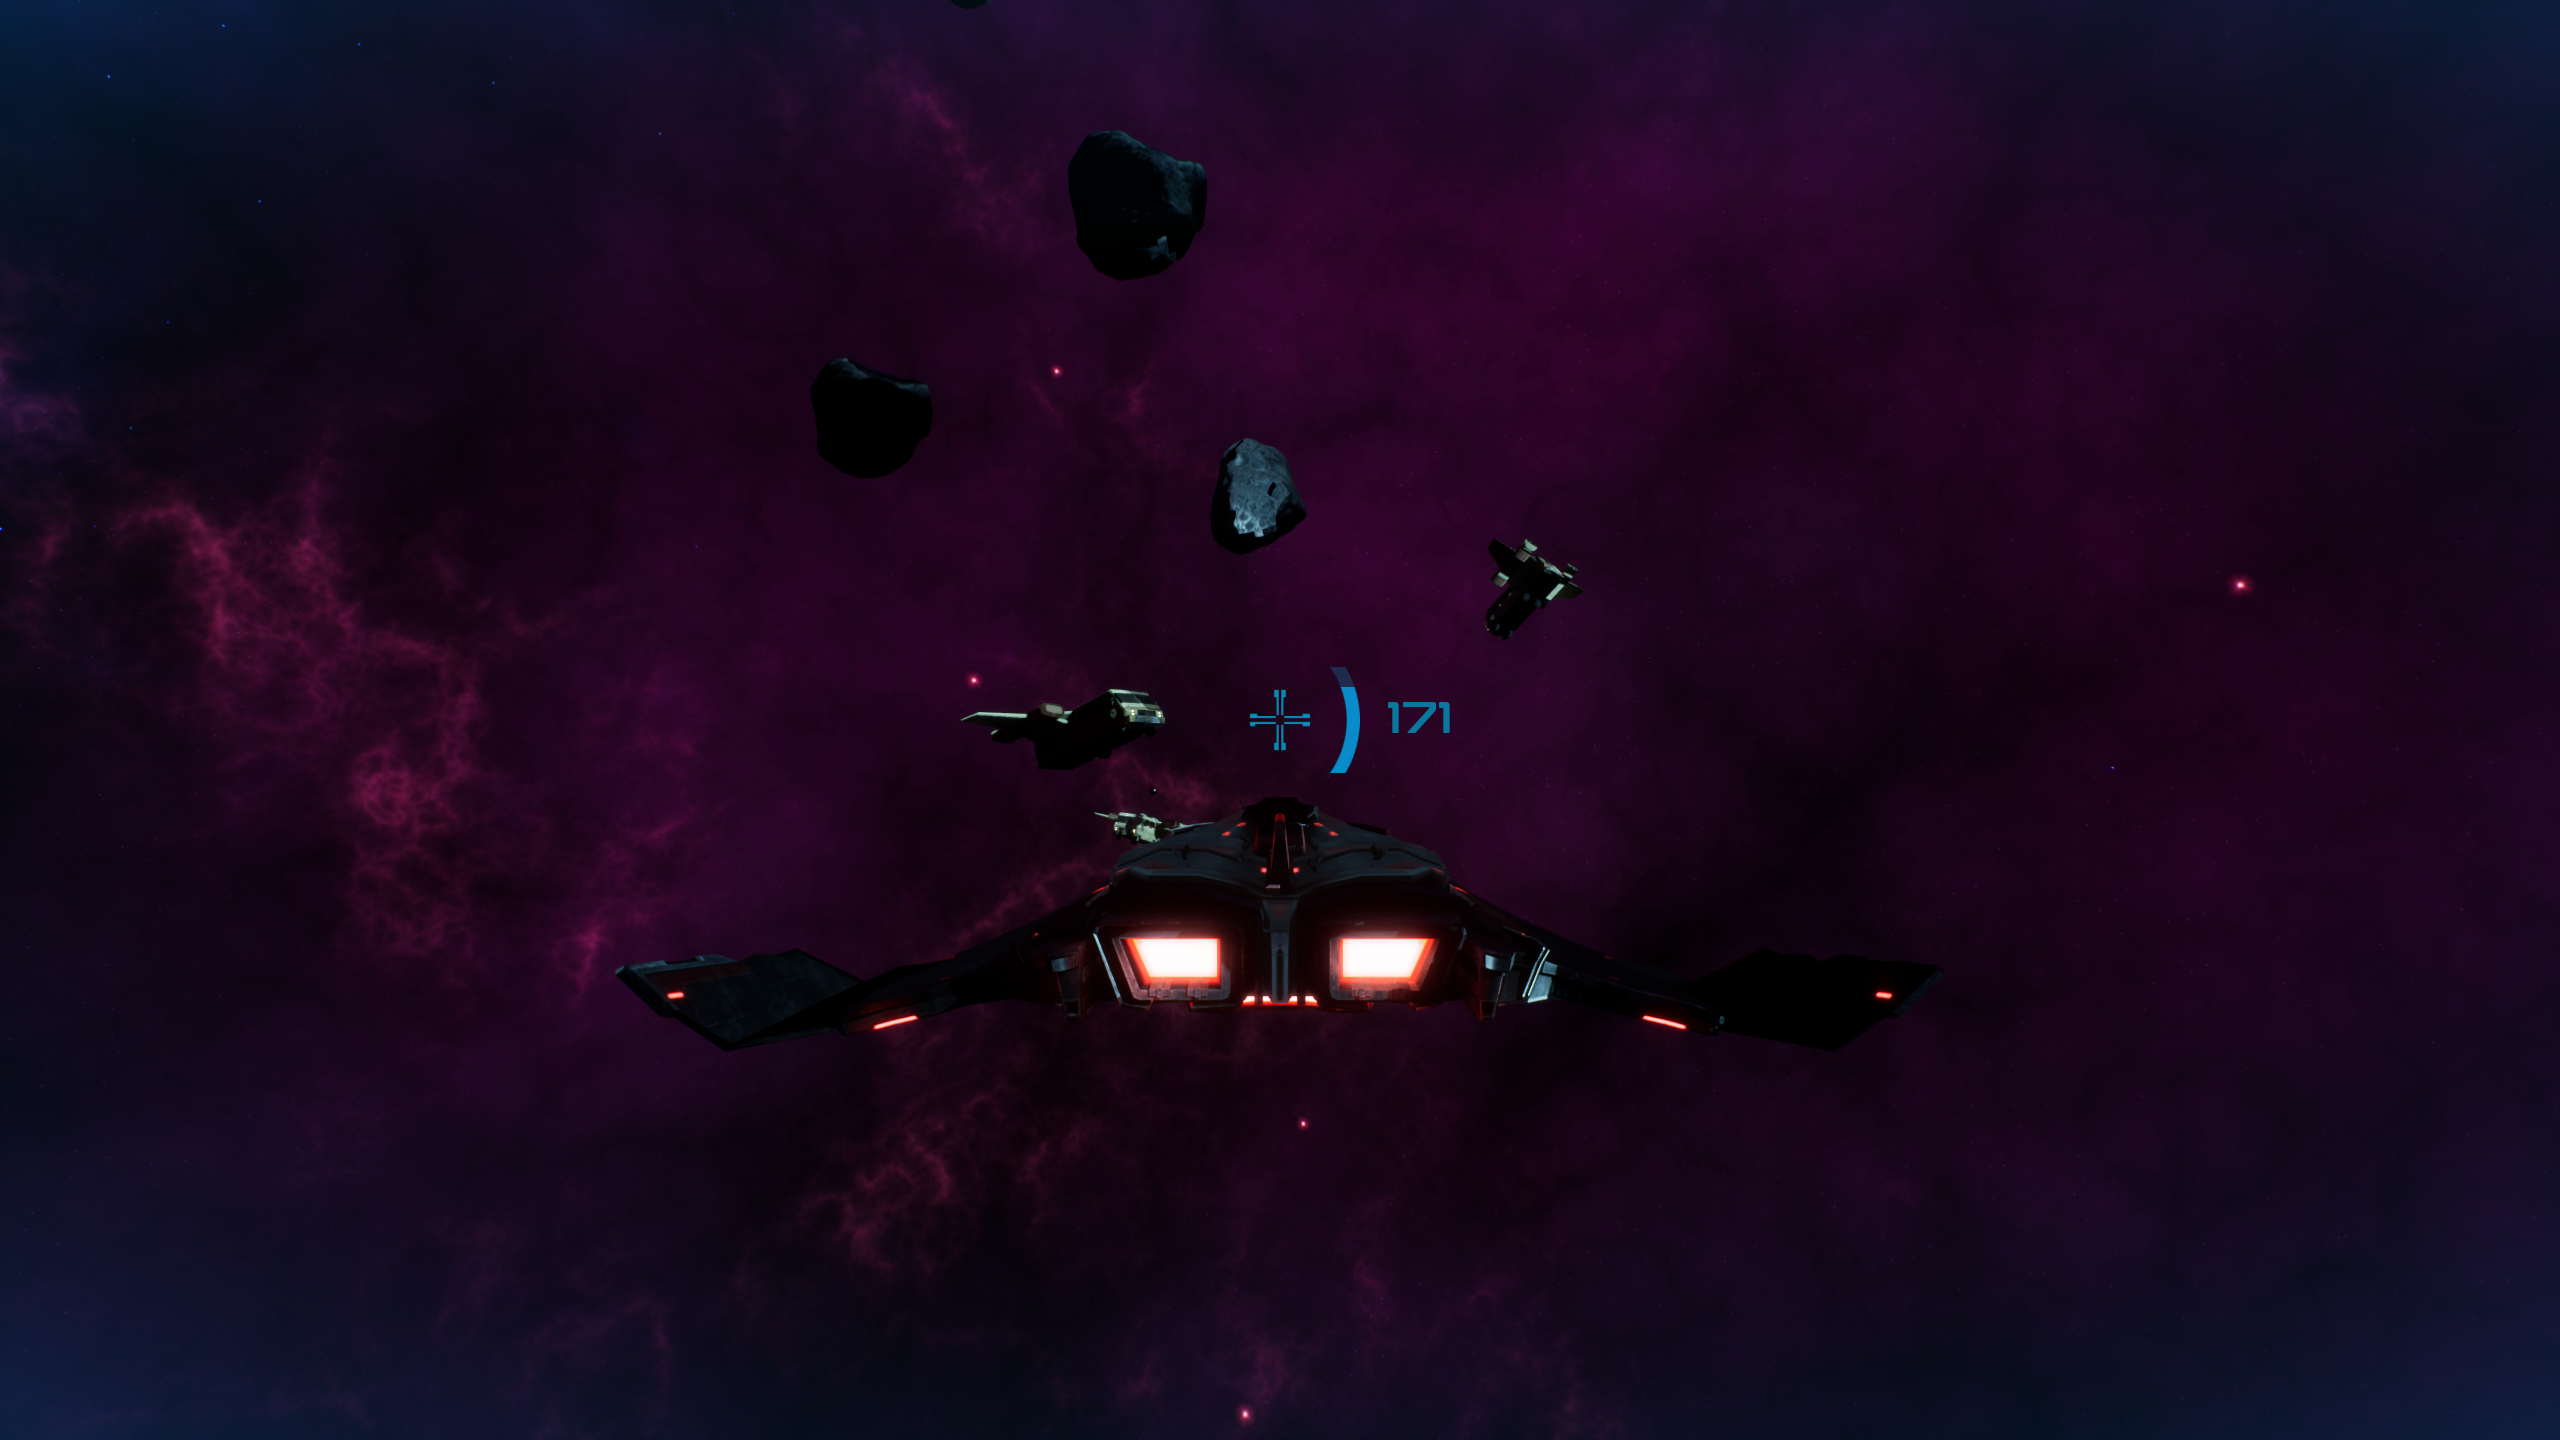
\includegraphics[width=1.0\textwidth]{images/astra004_gameplay.png}
	\caption{Snímek z verze 0.0.4}
\end{figure}
\clearpage

% BIBLIOGRAFIE, ZDROJE

\printbibliography[title={Seznam literatury a zdrojů}]
\addcontentsline{toc} {section} {Seznam užité literatury a zdrojů}

\end{document}
